\begin{frame}
  \frametitle{Molten Salt Reactor Designs}
  \begin{columns}
    \column{3cm}
    \begin{figure}
      \centering
      \footnotesize
      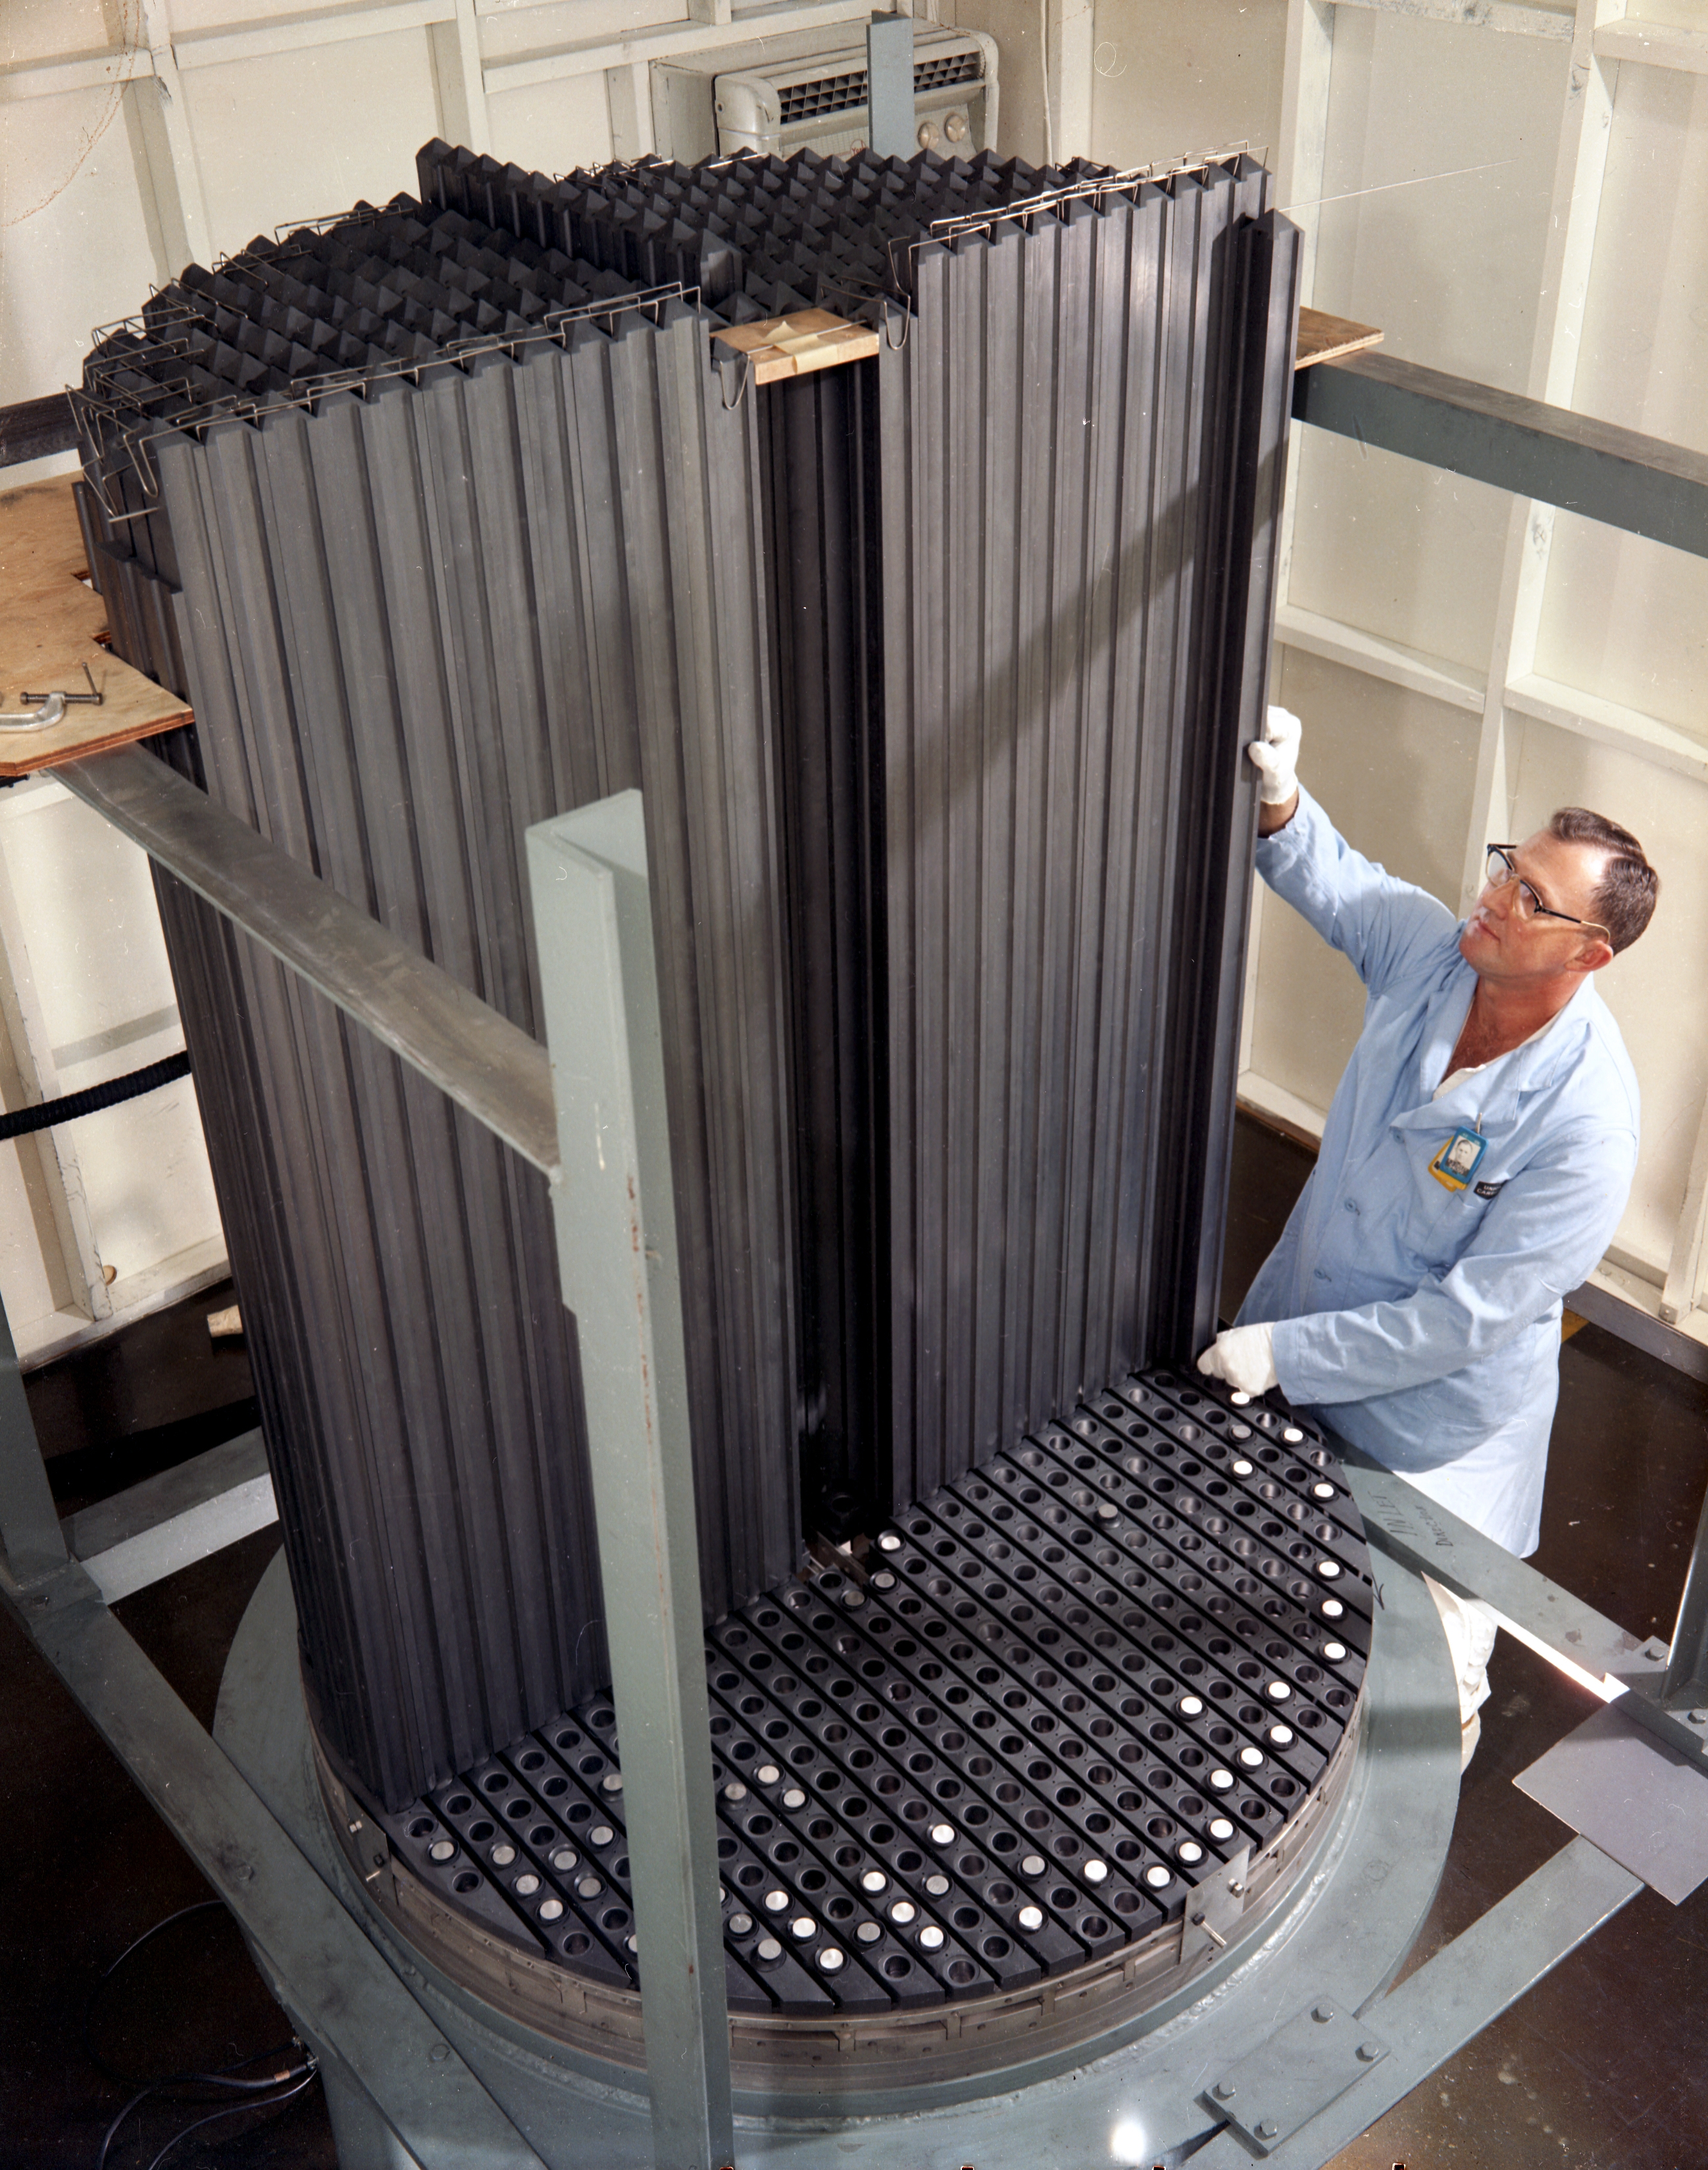
\includegraphics[width=\textwidth]{./images/msre-photo}
      \caption{Graphite assembly for the Molten Salt Reactor Experiment
      \cite{ornl_first-ever_2023}.}
    \end{figure}
    \column{7cm}
    \begin{table}
      \footnotesize
      \centering
      \caption{Thermal-spectrum MSR designs under active development.}
      \begin{tabular}{l l}
        \toprule
        Reactor & Organization \\
        \midrule
        Integral Molten Salt Reactor & Terrestrial Energy \\
        TMSR-LF & CAS (China) \\
        Compact Molten Salt Reactor & Seaborg Technologies \\
        Copenhagen Atomics Waste Burner & Copenhagen Atomics \\
        \bottomrule
      \end{tabular}
    \end{table}
    \begin{table}
      \footnotesize
      \centering
      \caption{Fast-spectrum MSR designs under active development.}
      \begin{tabular}{l l}
        \toprule
        Reactor & Organization \\
        \midrule
        Molten Chloride Fast Reactor & TerraPower \\
        Molten Salt Fast Reactor & CNRS (France) \\
        Stable Salt Reactor - Wasteburner & Moltex Energy \\
        Molten Chloride Salt Fast Reactor & Elysium Industries \\
        \bottomrule
      \end{tabular}
    \end{table}
  \end{columns}
\end{frame}

\begin{frame}
  \frametitle{Hybrid $S_N$-Diffusion Method: Literature Review}
  \textbf{Absorber Blackness} \\
  Encompasses a broad class of procedures for generating boundary conditions to match approximate
  solutions of low-order methods to more accurate solutions of high-order methods
  \cite{davison_influence_1951, spinks_extrapolation_1965, pellaud_extrapolation_1968,
  mendelson_two-dimensional_1969}. \\
  The boundary conditions are generalizations of the Marshak boundary condition, which in 1-D are
  of the form:
  %
  \begin{align}
    \frac{\phi(x)}{d\phi(x)/dx} =& \lambda \label{eq:marshak}
    \shortintertext{where}
    \phi =& \mbox{ neutron scalar flux,} \nonumber \\
    \lambda =& \mbox{ linear extrapolation length.} \nonumber
  \end{align}
  %
  Alternatively, the internal boundary conditions may be replaced with ``effective'' diffusion
  coefficients and absorption cross sections \cite{bretscher_computing_1997}.
\end{frame}

\begin{frame}
  \frametitle{Hybrid $S_N$-Diffusion Method: Literature Review}
  \textbf{Method of Equivalent Cross Sections (MECS)}
  \begin{columns}
    \column[t]{7cm}
    Implemented in the CITATION nodal diffusion code for control rod modeling in High-Temperature
    Gas-Cooled Reactors (HTGR). \\
    \textbf{Methodology}
    \begin{enumerate}
      \item Run a high-fidelity 1-D neutron transport calculation on a representative supercell of
        the control rod and its vicinity
      \item Match the net leakage rates from the transport solver to the diffusion solver using an
        analytic formula
      \item Solve for the equivalent diffusion coefficients
    \end{enumerate}
    \textbf{Limitations}
    \begin{enumerate}
      \item The solving procedure places geometric constraints on the geometry nodalization
      \item Incompatible with reactor geometries which contain control rods that are too close
      \item Only applicable for coarse-mesh diffusion solvers
    \end{enumerate}
    \column[t]{4cm}
    \begin{figure}
      \centering
      \includegraphics[width=.75\columnwidth]{../images/mecs-geometry}
      \caption{Geometry of the supercell (top) and the diffusion solver mesh (bottom)
        \cite{fen_modelling_1992}.}
    \end{figure}
  \end{columns}
\end{frame}

\begin{frame}
  \frametitle{Hybrid $S_N$-Diffusion Method: Literature Review}
  \textbf{Response-Based Methods}
  \vspace{.3cm}

  Another technique applied to modeling control rods in HTGRs with nodal diffusion codes. \\
  Uses neutron transport solutions to generate response functions, which relate flux-based
  quantities (e.g., incident partial currents $\Rightarrow$ average nodal flux and outgoing partial
  currents)
  \vspace{.3cm}

  \textbf{Examples}
  \begin{enumerate}
    \item Fen et al. \cite{fen_modelling_1992} developed the Response Matrix Method which generates
      boundary conditions from response functions.
    \item Rahnema et al. \cite{rahnema_advanced_2011} developed the integrated diffusion/transport
      (IDT) method which generates coupling coefficients used in nodal diffusion calculations.
  \end{enumerate}
\end{frame}

\begin{frame}
  \frametitle{Hybrid $S_N$-Diffusion Method: Proposed Work}
  \textbf{Investigate and rectify potential rod cusping errors}
  \vspace{.2cm}
  \begin{columns}
    \column[t]{6.5cm}
    Rod cusping occurs when the control rod boundary does not align perfectly with the mesh element
    boundaries when modeling time-dependent control rod insertion/withdrawal.
    \vspace{.1cm}
  
    Potential solutions:
    \begin{itemize}
      \item Adaptive meshing
      \item Approximate flux-volume weighting of cross sections
      \item Projection-based cusping treatment \cite{schunert_control_2019}
      \begin{itemize}
        \item Projection of piecewise constant cross sections onto a set of Legendre polynomials
        \item Exact integration of the FEM weak form is achieved
      \end{itemize}
    \end{itemize}
    \column[t]{5.5cm}
    \begin{figure}
      \centering
      \includegraphics[width=.65\columnwidth]{images/cusping}
      \caption{Illustration of control rod cusping effect.}
      \includegraphics[width=.65\columnwidth]{images/control-drum}
      \caption{Adaptive meshing of a rotating control drum.}
    \end{figure}
  \end{columns}
\end{frame}

